%----------------------------------------------------------------------------------------
%	Inställningar och dokumentkonfiguration
%----------------------------------------------------------------------------------------

\documentclass[paper=a4, fontsize=11pt]{report} % A4-sida och 11 punkters fontstorlek

\usepackage[T1]{fontenc} % 8-bitarskodning som har 256 glyfer
\usepackage[swedish]{babel} % Svenskt språk
\usepackage[utf8]{inputenc} % För svenska tecken
\usepackage{dtklogos} % Logos
\usepackage{wallpaper} % Bakgrundsbild
\usepackage{fancyhdr} % Specialsidhuvud och sidfot
\usepackage{enumerate} 
\usepackage{xifthen}% provides \isempty test
\pagestyle{fancyplain} % Använd sidhuvud och sidfot på alla sidor
\fancyhead[L]{Seminar 1 -- 1DV020 -- 2015 -- Server Administration} % Titel till vänster i sidhuvud
\fancyhead[C]{} % Tomt i mitten
\fancyhead[R]{} % Tomt till höger
\fancyfoot[L]{} % Tomt till vänster
\fancyfoot[C]{} % Tomt i mitten
\fancyfoot[R]{\thepage} % Sidnumrering till höger i sidfoten
\renewcommand\thesection{\arabic{section}} % Section beter sig som i dokumentklassen article

\newcommand{\win}[1]{Microsoft Windows Server\ifthenelse{\isempty{#1}}{}{ #1}}
\newcommand{\gui}[0]{``Server with a GUI''}
\newcommand{\core}[0]{Windows Server Core}
%----------------------------------------------------------------------------------------
%	TITLE SECTION
%----------------------------------------------------------------------------------------
\newcommand\BackgroundPic{
    \put(-50,-50){
    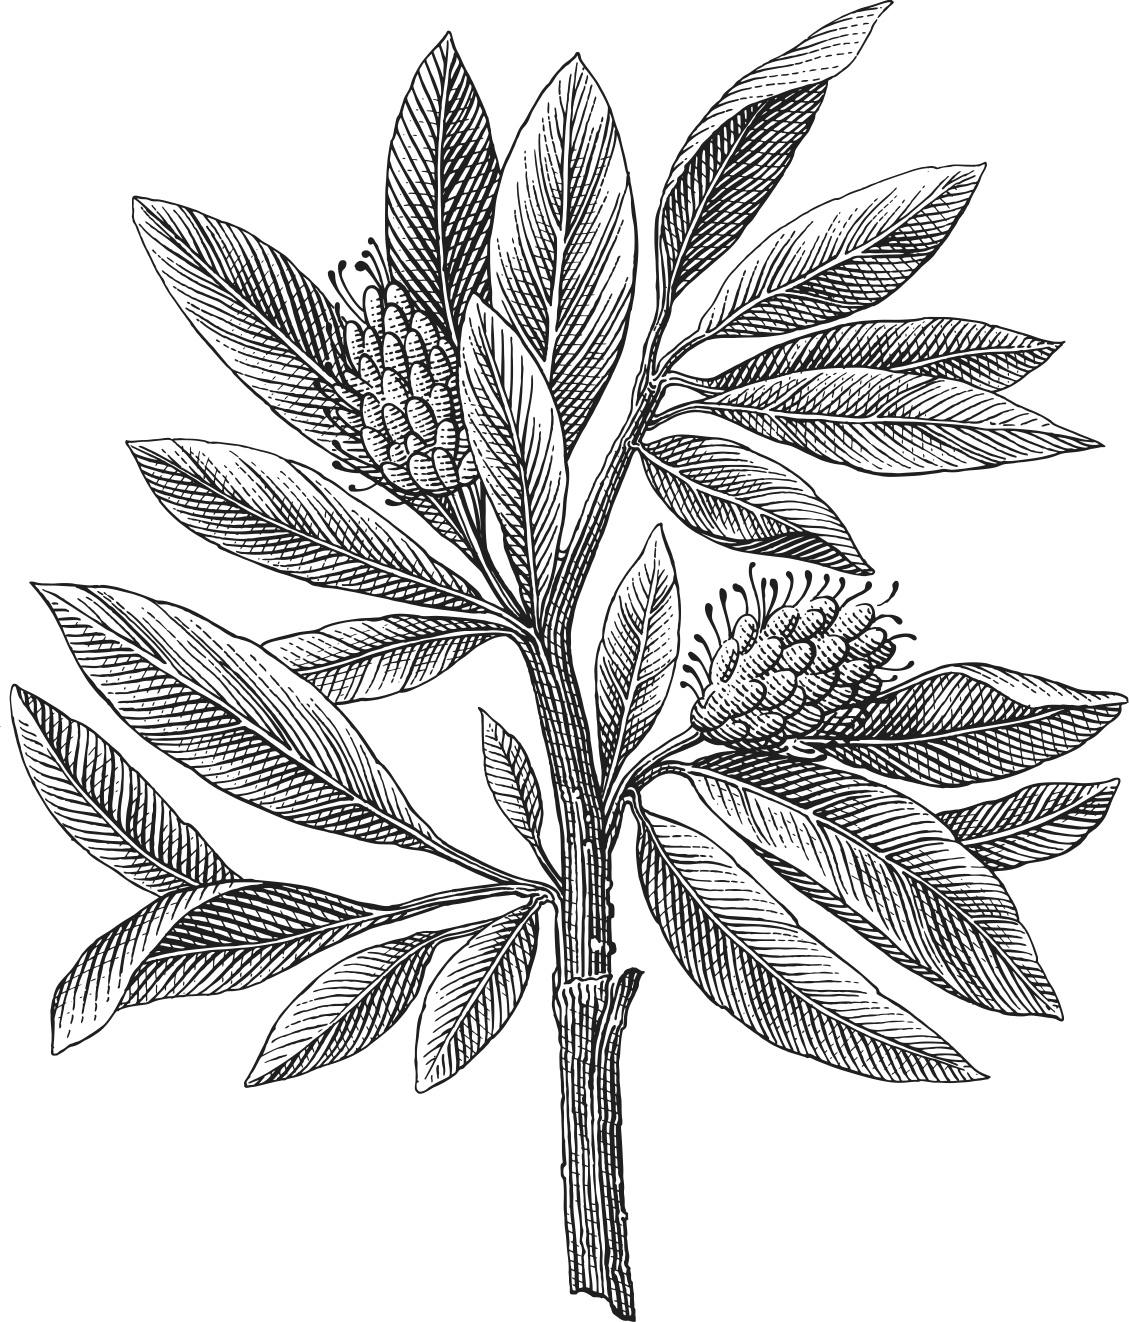
\includegraphics[keepaspectratio,scale=0.65]{lnu_etch.png} % Bakgrundsbild
    }
}
\newcommand\BackgroundPicLogo{
    \put(15,700){
    
\includegraphics[keepaspectratio,scale=0.10]{logo.png} % Logga i vänstra hörnet
    }
}

\newcommand{\horrule}[1]{\rule{\linewidth}{#1}} % Skapa hortisontell linje

\title{	\vspace{-10cm}
    \normalfont \normalsize
    \textsc{Linnaeus University} \\ [25pt] % Universitetes namn
    \horrule{0.5pt} \\[0.4cm] % Tunn linje högst upp
    \huge Seminar 1\\ % Arbetes titel
	\large \textcolor{gray}{1DV020 -- Server Administration}
    \horrule{0.5pt} \\[0.4cm] % Tunn linje längst ner
}

\author{Jacob Lindehoff} % Författarnas namn

\date{\normalsize\today} % Dagens datum

\begin{document}
\AddToShipoutPicture*{\BackgroundPic} % Lägger in backgrundsbild på första sidan
\AddToShipoutPicture*{\BackgroundPicLogo}
\maketitle % Skriv ut titeln
\noindent % Tabba inte in på första meningen

%------------------------------------------------
%	Introduktion
%------------------------------------------------
\section{Introduction}
During this seminar, we will address the following topics:
\begin{itemize}
\item Server vs. Client
\item Installation of various server operating systems
\item Post Setup
\item Basic configuration
\item Administrative Tools

\end{itemize}

%------------------------------------------------
%	Deadline
%------------------------------------------------
\section{Dealine}
The seminar is on the {\color{red}28th January 2015} and it is compulsory. If you cannot participate, it must be notified in advance and a written report of the seminar must be submitted no later than {\color{red}3 days} after the seminar. The written report should contain detailed answers to all questions in the seminar.
\newpage
%------------------------------------------------
%	Seminariefrågor
%------------------------------------------------
\section{Seminar Questions}

\begin{enumerate}
\begin{large}
\item Vad är det som gör en datorn till en server (Hårdvaran)?
\item Vad menas med en server när man pratar om en mjukvara?
\item Vilka är de stora milstolparna i \win{} historia?
\item Beskriv det olika typerna av administrationsroller som finns och vilken du är mest intresserad av att arbeta som?
\item Du har en kund som har 50 klienter, de vill köra \win{2012 R2} och serven ska användas som filserver.
\begin{enumerate}[a.]
\item Hur gå du till väga för att hitta lämplig hårdvara till företaget? 
\item Vilken hårdvara rekommenderar du?
\end{enumerate}
\item Vad är viktigt att tänka på innan du installerar \win{}?
\item Vad är HCL och varför ska den kontrolleras innan man installerar Windows Server?
\item Hur skiljer sig installations förfarandet av \win{2003} och \win{2008/2012}?
\item Client Access Licenses
\begin{enumerate}[a.]
\item Vilka är de olika CAL som Microsoft har?
\item Hur fungerar dessa?
\item Hur väljer man rätt CAL, i vilka scenarion passar de olika CAL?
\end{enumerate}
\item Microsoft har oftast haft många olika versioner av sitt serveroperativsystem, detta är dock något de har ändrat i \win{2012}. \\ 
Vilka versioner finnas av följande operativsystem och hur skiljer sig de åt.
\begin{enumerate}[a.]
\item \win{2008 R2}
\item \win{2012 R2}
\end{enumerate} 
\item \core
\begin{enumerate}[a.]
\item Vad är \core?
\item I vilka scenarion passar det att använda en \core{} installation?
\item Vilka fördelar har en \core{} installation jämfört med en \gui?
\end{enumerate}
\item Vad ingår i en Post Setup?
\begin{enumerate}[a.]
\item Hur går Post Setup till i \gui
\item Hur går Post Setup till i \core
\end{enumerate}
\item Nämn några bra Nätverkskommandon och vad de används till?
\item Vilka användbara kommandon i \core{} har du lärt dig hittills?
\item Vad används följande administrationsverktyg till:
\begin{enumerate}[a.]
\item Loggboken
\item Enhetshanteraren 
\item Diskhanteraren
\item Tjänster
\end{enumerate}
\item Vad är Microsoft Management Console och hur använder man den?
\item Vad är Powershell, kortfattat, vi har en hel kurs i detta LP4?

\end{large}
\end{enumerate}
\end{document}
